\documentclass[paper=a1,pagesize,parskip=half-,fontsize=24.88pt]{scrartcl}
\usepackage[utf8]{inputenc}
\usepackage[T1]{fontenc}
\usepackage[ngerman]{babel}
%skalierbare fonts
\usepackage{lmodern}
\usepackage{newpxmath}

%angenehmeres typsetting
\usepackage{microtype}

%fuer urls
\usepackage{url}

\usepackage{xcolor}

%mehrspaltig
\usepackage{multicol} 
\columnsep=70pt 
\columnseprule=3pt 

%grafiken einbinden
\usepackage{graphicx}
%schoene tabellen
\usepackage{booktabs}
%seitengeometrie
\usepackage{geometry}
\geometry{margin=4cm,top=4cm}
%blindtext
\usepackage{blindtext}
%erweiterte tabellenumgebung
\usepackage{tabularx}

%listings einbetten
\usepackage{listings}

\begin{document}

%minipages zum einfangen von layouts
\begin{minipage}[b]{0.74\linewidth}
  \huge\textbf{Eine unnötig komplizierte Abhandlung}\\[1cm]
  \huge{Untersuchung einer Sache von wirklichem Wert}\\[2cm] 
  \huge\textbf{Andy Weisen}\\[0.5cm]
  \Large Hochschule Bremerhaven\\[0.4cm]
  \Large\texttt{https://informatik.hs-bremerhaven.de/step2019/}\\
\end{minipage}
%
%eine zweite minipage rechts neben der vorigen, [t]op ausrichten
\begin{minipage}[t]{0.25\linewidth}
%grafik einbinden mit expliziter breite

\includegraphics[width=14cm]{Thunderlogo}\\
\end{minipage}

%mehrspaltige umgebung ohne ausgleich (ohne *: mit ausgleich)
\begin{multicols*}{3}

%section mit Sternchen werden nicht numeriert  
\section*{Einleitung}
\blindtext[1]

%grafik, die volle spaltenbreite fuellt
%png oder pdf Dateien erlaubt
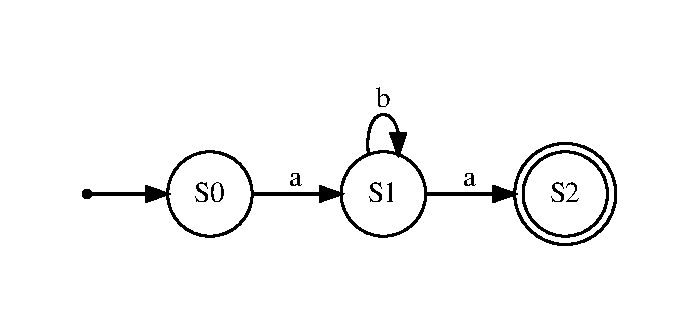
\includegraphics[width=\linewidth]{fsm}

\section*{Zielstellung}
\blindtext[1]
%align* umgebung fuer math
\begin{align*}
  \lim_{h\to 0}\frac{f(x+h)-f(x)}{h}
\end{align*}
\begin{align*}
    f_n=\begin{cases}
      a  & \text{if \(n=0\)} \\
      r\cdot f_{n-1} &\text{else}
    \end{cases}
\end{align*}
Im Mathemodus spielt \LaTeX{} gewisse Stärken aus.\footnote{
In Anlehnung an \url{http://tug.ctan.org/info/undergradmath/undergradmath.pdf}
}

\section*{Materialien}
\blindtext[1]

\vspace*{1cm}
%listings als code - nicht als screenshots ...
\begin{lstlisting}[language=bash,caption={Ein Listing},captionpos=b,frame=tb]
#!/bin/bash
for i in {1..10}; do
  echo $i
done
\end{lstlisting}

\blindtext[1]


\section*{Umsetzung}
\blindtext[1]

%tabularx{Gesamtbreite}{...} X-Spalten werden optimiert
% &  : trennt Einträge
% \\ : beendet eine Zeile
\begin{tabularx}{\linewidth}{XXX}
\toprule
\textbf{Zweck} & \textbf{Werkzeug} & \textbf{Ausgabe} \\
\midrule
Daten    & gnuplot      & svg,png,pdf \\
Graphen  & graphviz,dot & svg,png,pdf \\
Textsatz & \LaTeX{}     & pdf \\
\bottomrule
\end{tabularx}


\section*{Ergebnisse}
\blindtext[1]

  \begin{description}
    \item[STEP] Studieneingangsprojekt für die Studiengänge Informatik und Wirtschaftsinformatik.
    \item[SWE~I] ...
    \item[Mathe] ...
    \item[Prog~I] ...
    \item[Graphen] ...
  \end{description}

%vertikalen abstand auffuellen
\vfill

\includegraphics[width=\linewidth]{logo}
\vfill
Und jetzt sind Sie dran...
\end{multicols*}
\end{document}
